\section{Evidence So Far}
\label{sec:evidence}

본 결합 실험 전에 구성 요소마다 사전 등록한 작은 실험을 돌렸다(\cref{tab:evidence}). 표본이 작고 대부분 한 과제(머그를 트레이에)이므로 모든 값은 주황의 초기값이다. 각 결과가 바꾼 설계 결정을 함께 적는다. 공개 실물 데이터의 소규모 학습 시험처럼 파이프라인 확인이 목적이었던 값은 결과로 쓰지 않고 부록에만 둔다(\cref{sec:supp_tests}). \cref{fig:evidence}는 상위 자리의 위치 읽기를 같은 인터페이스에서 한눈에 비교한다.

\begin{figure}[t]
\centering
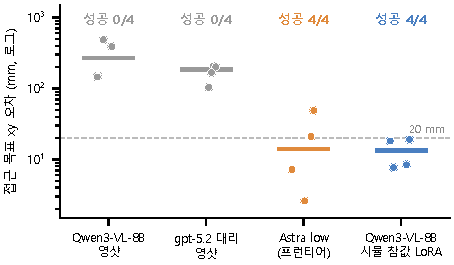
\includegraphics[width=\linewidth]{figures/evidence.pdf}
\caption{\textbf{상위 자리의 위치 읽기 (초기값).} 같은 동기 단독 인터페이스(\texttt{astra-solo@v2})로 머그-트레이 DEV 4편(시드 0·1 $\times$ standard·DR)을 돌렸을 때, 편마다 명령한 접근 목표의 xy 오차 중앙(점)과 네 편의 중앙(막대). 위의 숫자는 폐루프 성공이다. Astra는 파일럿 4편의 값이다(전체 팔 첫 3편도 성공해 합 7/7). 미세조정 8B는 시뮬 참값 라벨로 LoRA 학습한 판이다. 영샷 두 모델은 대상 위치를 10--50\,cm 틀리게 읽었고, 미세조정 8B는 Astra와 같은 범위로 들어왔다. 대리 모델(gpt-5.2)의 값은 오픈 모델 자체의 값이 아니다. 편 수가 4라 방향만 본다. 모든 값은 \tentative{초기값}이다.}
\label{fig:evidence}
\end{figure}


\begin{table*}[t]
\centering
\scriptsize
\setlength{\tabcolsep}{3pt}
\begin{tabular}{@{}p{0.17\linewidth}p{0.27\linewidth}p{0.30\linewidth}p{0.20\linewidth}@{}}
\toprule
질문 & 조건 & 결과 (모두 초기값) & 바꾼 결정 \\
\midrule
상위 단독으로 조종할 수 있는가 & Astra low, 동기, Astra에 맞춘 인터페이스, 머그-트레이 DEV & \tentative{7/7}(파일럿 4/4 + 전체 팔 3/3); 파일럿 편당 \tentative{9--17}호출, 성공당 \tentative{591.5원}, 벽시계 \tentative{74--215\,s}; 무효 답 \tentative{0/44} & 결합 비교에 강한 기준선(AS) 추가 \\
영샷 오픈급 모델이 대신할 수 있는가 & 같은 인터페이스, Qwen3-VL-8B 5편, gpt-5.2 대리 4편 & \tentative{0/5}, \tentative{0/4}; 대리의 접근 목표 xy 오차 편 중앙 \tentative{104--207\,mm}(Astra \tentative{2.6--48.9\,mm}) & 영샷 대체 불가, 학습이 전제 \\
학습한 8B 상위 모델 & 시뮬 참값 라벨 LoRA, TRAIN 300편, 2 에폭, \tentative{1.39} GPU-h & 접근 오차 \tentative{125.5$\rightarrow$2.6\,mm}, 그리퍼 행동 \tentative{0.32$\rightarrow$0.95}; 폐루프 DEV \tentative{4/4}(영샷 \tentative{0/4}); p50 \tentative{3.5\,s}(Astra \tentative{6.8\,s}) & H-L의 첫 근거, 다양화·OOD로 확장 \\
상위 한 호출은 정확한가 & Isaac 벤치, 계획대로 30장 + 틀어진 20장, v1·v2·축 덧그림 & 수정 방향 \tentative{13/13}, 7--10\,cm 목표 어긋남 알아채기 \tentative{0/13}; v2 채택(\tentative{+0.20} [\tentative{+0.05, +0.40}]) & 병목은 알아채기; 예상 상태는 청크 기반으로 \\
결합 흐름의 상수 & Astra low, 흐름 F0/F1 각 3편, 정지 파지 판정 40장 & 답까지 p50 \tentative{8.9/10.0\,s}, 호출당 \tentative{49.7/58.0원}; 실제 쥠 놓침 \tentative{13/25}; 부드러운 반영 저크 \tentative{0.83} 대 \tentative{2.36\,m/s$^3$} & 형식 F0, 답 나이 상한 15\,s, 확정은 T1·V1h \\
VLA 단독이 의미가 있는가 & 결합 사전 실행 DEV 12편 + 5조건(재생 1.0·0.75·0.5배) & 모든 조건 \tentative{0/12}(규칙 기준선 \tentative{12/12}); 12편 중 \tentative{8}편은 런타임 멈춤 고리 & 유료 결합 전 런타임 수정·VLA 관문 \\
결정이 실행을 조종하는가 & 강제 결정 반사실 준수(우연 약 0.33) & 학습 없이 \tentative{0.431}(시뮬); 먼 구간 분기로 시뮬 \tentative{0.344$\rightarrow$0.991}, 실데이터 \tentative{0.339$\rightarrow$0.536} & 먼 구간 결정 경유는 시뮬 판만 \\
호출 신호 & VLA 백본 특징 새로움, 결정 확신도 & 새로움 큰 오류 AUROC \tentative{0.570}; 확신도 \tentative{0.804}, 새 표본 실데이터 \tentative{0.748}(문턱 0.75) & 둘 다 게이트로 쓰지 않음, 확신도는 기록만 \\
\bottomrule
\end{tabular}
\caption{\textbf{지금까지의 근거.} 모든 실험은 판정 기준을 실행 전에 고정했다. 값은 작은 표본의 초기값이며 본 결과가 아니다. 대리 모델(gpt-5.2)의 값은 오픈 모델 자체의 값이 아니다.}
\label{tab:evidence}
\end{table*}

\paragraph{Astra에 맞추면 상위 단독 조종은 된다.} 처음의 탐침에서 Astra 단독 조종은 \tentative{0/6}이었다. 그러나 그 조건은 Astra에 불리했다(결함 있는 프롬프트, 5\,cm 이하 수정만 허용, 기다리지 않는 흐름). 비교의 각 팔은 그 방법에 최적인 조건으로 설계해야 한다. 그래서 로봇이 답을 기다리고, 절대 말단 목표를 내며, 머리 영상에 탁자면 좌표 격자를 그리고, 판정 개념·축·카메라 자세를 정의한 인터페이스로 다시 쟀다. 같은 Astra가 \tentative{7/7}을 성공했다. 탐침의 0/6은 실력이 아니라 조건의 값이었다. 이 결과로 Astra에 맞춘 단독 팔을 결합 비교의 강한 기준선으로 더했다. 결합 계층은 이 기준선 앞에서 성공률뿐 아니라 로봇이 멈추는 시간과 비용으로도 비교된다. 단독 팔 벽시계의 대부분은 답을 기다리는 시간이다.

\paragraph{영샷 오픈급 모델은 위치를 읽지 못한다.} 같은 인터페이스에 로컬 Qwen3-VL-8B를 넣으면 \tentative{0/5}였고, 학습 가능 크기의 오픈 목표와 공개 지표가 비슷한 OpenAI 대리 모델(gpt-5.2)도 \tentative{0/4}였다. 네 편 모두 접근 단계에서 끝났고, 명령한 접근 목표가 머그에서 편 중앙 \tentative{104--207\,mm} 떨어졌다. 격자의 깊이 방향을 12--19\,cm 멀게 읽은 것이 주원인이다. 사전 등록 판정은 ``인식''이다. 대리 모델은 $n=4$이고 오픈 모델 자체가 아니므로 방향만 본다.

\paragraph{학습한 8B 상위 모델: H-L의 첫 근거.} 35B는 학습 시간이 길어, 8B로 경향부터 봤다. Qwen3-VL-8B를 동기 단독 형식의 시뮬 참값 라벨로 LoRA 학습했다(에폭당 \tentative{6,521} 표본, H200 한 장 \tentative{1.39} GPU-h). 오프라인 DEV에서 접근 목표 xy 오차 중앙이 \tentative{125.5\,mm}에서 \tentative{2.6\,mm}로 줄었고, 그리퍼 행동 정확도는 \tentative{0.32}에서 \tentative{0.95}로 올랐다. 폐루프 DEV 4편은 \tentative{4/4}(편당 6호출)였고, 같은 한도의 영샷 8B는 \tentative{0/4}였다. 지연은 p50 \tentative{3.5\,s}로 Astra(\tentative{6.8\,s})의 약 절반이고 API 비용은 0이다. 영샷 실패의 원인이던 위치 읽기가 무료 시뮬 참값의 촘촘한 감독으로 메워진다는 점에서 H-L의 첫 근거로 본다. 한계는 분명하다. $n=4$이고, DEV는 학습과 같은 분포이며, 라벨은 Astra가 아니라 시뮬 참값이다. 지연은 ``빠르다'' 기준(p50 $\le$2\,s)에 아직 못 미친다. 또 이 형식은 결합 규약의 구간 의도를 담지 않는다. 35B 크기 효과와 일반성에 대해서는 말하는 것이 없다.

\paragraph{상위 한 호출의 공백: 알아채기.} VLA는 상위가 옳다는 전제로 움직이므로 상위 한 호출의 정확도를 먼저 쟀다. 오라클 계획기를 반속도로 돌린 Isaac 벤치에서 계획대로인 스냅숏과, 7--10\,cm 옆의 엉뚱한 곳·엉뚱한 물체·엉뚱한 놓을 곳에 멈춘 스냅숏을 찍었다. 도착 시점의 오라클 방향으로 채점했다. Astra가 수정을 낸 경우 방향은 \tentative{13/13} 맞았다. 그러나 엉뚱한 곳과 놓을 곳에 멈춘 상태는 세 프롬프트 판 모두 \tentative{0/13}으로 알아채지 못하고 ``진행 중, 의도와 맞음''이라 답했다. 엉뚱한 물체는 v2 \tentative{5/7}, 로봇 기준 축을 덧그린 판 \tentative{7/7}로 잡았다. 구간 계획을 더한 v2 프롬프트를 채택했다. 알아채기를 올리려는 시도는 둘 다 넣지 않았다. effort medium은 \tentative{1/13}이었다. ``목표를 확인하라''는 문장은 \tentative{7/13}까지 올렸지만 계획대로인 상태에서 괜한 수정을 냈다. 괜한 수정은 요청에 실은 ``도착 예상 손끝''이 최근 속도를 9\,s 넘게 외삽한 값이라 크게 튄 탓이었다. 그래서 결합의 예상 상태를 확정 청크 기반으로 바꾸었다(\cref{sec:protocol}). 이 공백은 H-L의 ``더 좋다'' 기준이 겨누는 곳이기도 하다.

\paragraph{VLA 단독 \tentative{0/12}의 분해.} 결합의 무료 사전 실행(로컬 VLM을 상위 대역으로)은 배관을 통과했다. 충돌이 없었고, 동시 요청 1개 불변식이 유지되었으며, 늦은 답은 폐기되었다. 그러나 VLA 단독이 \tentative{0/12}여서, 짝 비교의 기준 팔이 바닥이면 결합의 이득을 가를 수 없다. 기존 기록으로 나눠 보니 \tentative{8}편은 VLA가 아니라 런타임의 멈춤 고리였다. 고유 감각 모순이 확정 보류를 부르고, 보류가 결정을 비워 청크가 멈춘 채 같은 모순이 이어졌다. 나머지 \tentative{4}편은 머그를 쳐서 떨어뜨리거나 머그 위 약 10\,cm에서 내려가지 못한 VLA 자체 실패였다. 뒤이은 무료 실험에서 VLA 단독은 모든 조건(두 확정 규칙, 재생 속도 1.0·0.75·0.5배)에서 \tentative{0/12}였다. 같은 장면의 스크립트 규칙 기준선은 \tentative{12/12}였다. 느린 재생은 지나침을 \tentative{87.7$\rightarrow$17.9\,mm}로 줄였지만 성공은 늘지 않아 채택하지 않았다. 이 결과로 유료 결합 실험 앞에 런타임 수정과 VLA 단독 관문을 두었다(\cref{sec:plan}). 오프라인 준수 지표로 체크포인트를 고르고 폐루프 성공을 보지 않은 채 짝 비교를 설계한 것이 절차상의 틈이었다.

\paragraph{결정이 실행을 조종하게 하기.} 학습 없이 전문가의 조건만 바꾼 진단에서 강제 방향 준수는 우연 수준이었다(시뮬 \tentative{0.431}, 우연 약 0.33). 반면 그리퍼 사건과 인과로 묶인 단계 토큰은 \tentative{0.95}로 따랐다. 결정 드롭아웃과 추론 때의 분류기 없는 안내는 준수를 거의 올리지 못하고 청크와 그리퍼를 무너뜨렸다(최고 \tentative{0.598}, 비열등 실패). 먼 구간 반사실 분기를 50\% 섞자 시뮬(R2)에서 먼 구간 준수가 \tentative{0.344}에서 \tentative{0.991}로 올랐다. 분기를 만들지 않은 과제에서도 \tentative{0.979}였고, 접촉 근처 능력은 비열등했다. 대가는 먼 구간 청크 오차 \tentative{+29\%}다. 같은 레시피를 공개 실물 데이터에 옮기면 \tentative{0.536}에 그쳤다. 학습 편과 검증 편의 준수가 같아(\tentative{0.549/0.523} 대 \tentative{0.552/0.521}) 일반화 간극이 아니라 과소적합이며, 더 긴 학습과 분기 비율을 시험 중이다.

\paragraph{쓰지 않기로 한 것.} 흐름 호출을 거르는 신호로 VLA 백본 특징의 새로움을 시험했다. 모델 자신의 큰 오류를 AUROC \tentative{0.570}으로만 갈라 쓰지 않는다. 판정 밖 기준선인 결정 확신도는 \tentative{0.804}였지만, 새 표본에서 다시 재니 실데이터 \tentative{0.748}로 문턱(0.75)에 못 미쳤다. 운용 모의에서는 트리거가 거의 늘 켜졌다. 그래서 확신도는 결정마다의 ``선택 이유'' 기록으로만 둔다. 우리 모델의 오류는 낯선 장면보다 익숙한 장면 안의 모호함에서 났다. MolmoAct식 학습 보강(미래 손끝 궤적 보조 손실, 층별 KV 조건, 명령을 VLA 입력에 보여 주기)도 사전 등록 문턱을 넘지 못했다(부록 \cref{sec:supp_tests}). 원 논문의 성립 조건(보정된 카메라, 조건을 관측과 독립으로 바꾼 데이터)을 갖추기 전에 겉모양만 옮긴 탓이 섞여 있어, 이식 전에 성립 조건을 관문으로 먼저 확인하는 절차를 넣었다.
